%%%%%%%%%%%%%%%%%%%%%%%%%%%%%%%%%%%%%%%%%%%%%%%%%%%%%%%%%%%%%%%%%%%%%%%%%%%
\chapter{Étude de la viabilité financière et plan d'exécution}
\label{Chapitre_5}
%%%%%%%%%%%%%%%%%%%%%%%%%%%%%%%%%%%%%%%%%%%%%%%%%%%%%%%%%%%%%%%%%%%%%%%%%%%
\section{Introduction}
\label{sec:intro_chap5}
%%%%%%%%%%%%%%%%%%%%%%%%%%%%%%%%%%%%%%%%%%%%%%%%%%%%%%%%%%%%%%%%%%%%%%%%%%%

Les chapitres précédents ont successivement démontré que Vocallia répondait à un besoin de marché identifié et quantifié (chapitre~2), qu'il pouvait être structuré en un modèle commercial scalable et défendable (chapitre~3), et qu'il reposait sur une architecture technique réalisable, résiliente et conforme aux contraintes réglementaires locales (chapitre~4). Reste un dernier test, le plus exigeant aux yeux d'un jury comme d'un investisseur~: la viabilité financière. Une opportunité de marché, aussi réelle soit-elle, ne se transforme en entreprise pérenne que si la trajectoire économique projetée est cohérente, les hypothèses calibrées avec prudence, et les jalons d'exécution alignés sur la capacité d'investissement disponible.

L'objet de ce chapitre n'est pas de chiffrer des coûts ou des revenus pour eux-mêmes, mais d'évaluer dans quelles conditions Vocallia peut franchir, sans rupture financière, la séquence MVP~$\to$~pilote~$\to$~production identifiée au chapitre~4, tout en restant fidèle aux fondations du modèle économique posées au chapitre~3. L'analyse procède en trois temps. Elle pose d'abord les hypothèses financières structurantes, l'investissement initial nécessaire et la structure de coûts d'exploitation. Elle construit ensuite des projections de revenus, un compte de résultat prévisionnel et un seuil de rentabilité, déclinés selon trois scénarios — prudent, central et ambitieux — afin de tester la robustesse du modèle. Elle examine enfin le plan de financement, les indicateurs de rentabilité, le plan d'exécution opérationnelle, l'impact attendu et la cartographie des risques.

Toutes les valeurs chiffrées de ce chapitre sont présentées comme des \emph{estimations indicatives}, à valider à mesure de l'avancement du projet. Elles s'appuient sur les coûts unitaires établis au chapitre~4 — coût variable d'environ 0{,}27~DT par appel de deux minutes, soutenant une marge brute de l'ordre de 65~\% sur le palier Starter — et sur des hypothèses prudentes pour une clientèle PME tunisienne en phase d'amorçage. Lorsque les données disponibles ne permettent pas un calcul rigoureux, les éléments sont présentés comme des hypothèses à valider, et non comme des certitudes. Cette discipline est, in fine, la meilleure défense du chapitre~: un plan financier crédible n'est pas un plan optimiste, c'est un plan dont chaque chiffre peut être discuté, contesté et défendu.

%%%%%%%%%%%%%%%%%%%%%%%%%%%%%%%%%%%%%%%%%%%%%%%%%%%%%%%%%%%%%%%%%%%%%%%%%%%
\section{Hypothèses financières et cadre de projection}
\label{sec:hypotheses_financieres}
%%%%%%%%%%%%%%%%%%%%%%%%%%%%%%%%%%%%%%%%%%%%%%%%%%%%%%%%%%%%%%%%%%%%%%%%%%%

\subsection{Logique de lancement et horizon de projection}
\label{subsec:logique_lancement}

L'horizon retenu pour la projection financière est de \textbf{36~mois} à compter du lancement opérationnel, en cohérence avec la trajectoire commerciale modélisée au chapitre~3 et avec la trajectoire technique du chapitre~4 (MVP~$\to$~pilote~$\to$~production). Trois raisons justifient cet horizon. D'abord, il correspond à la durée typique d'un cycle d'amorçage SaaS B2B, suffisamment long pour observer une trajectoire de revenus récurrents mais suffisamment court pour rester crédible sans extrapolation hasardeuse. Ensuite, il coïncide avec la fenêtre concurrentielle de 18 à 36~mois identifiée au chapitre~2~: c'est dans cet intervalle que Vocallia doit chercher à convertir son avance temporelle en actifs durables. Enfin, il permet de séquencer les jalons financiers de manière lisible — couverture progressive des charges fixes, équilibre opérationnel, et, à terme, génération éventuelle de cash réinvestissable.

\subsection{Hypothèses financières clés}
\label{subsec:hypotheses_cles}

L'ensemble des projections du chapitre repose sur un socle d'hypothèses explicitement formulées et reliées aux chapitres antérieurs. Le tableau~\ref{tab:hypotheses_financieres} les synthétise.

\begin{table}[H]
\centering
\caption{Hypothèses financières clés — Vocallia (horizon 36 mois)}
\label{tab:hypotheses_financieres}
\begin{tabular}{|p{4.5cm}|p{5cm}|p{5cm}|}
\hline
\textbf{Catégorie} & \textbf{Hypothèse retenue} & \textbf{Source / justification} \\
\hline
Plan d'entrée Starter & 79~DT/mois pour 100 appels inclus & Chapitre~3, section~3.8 \\
\hline
Prix unitaire effectif Starter & $\sim$0{,}79~DT par appel & Forfait~/~appels inclus \\
\hline
Coût variable moyen par appel (2~min) & $\sim$0{,}27~DT & Chapitre~4, structure de coûts API \\
\hline
Marge brute du plan Starter & $\sim$65~\% & Calcul direct $(0{,}79 - 0{,}27)/0{,}79$ \\
\hline
ARPU pondéré (mix des 3 paliers) & $\sim$120~DT/mois & Chapitre~3, section~3.9 \\
\hline
Contribution moyenne par client actif & $\sim$78~DT/mois & ARPU~$\times$~marge brute \\
\hline
Churn mensuel cible & 5 à 8~\% & Hypothèse prudente pour clientèle PME en amorçage \\
\hline
LTV/CAC visé & supérieur à 3~:~1 & Seuil minimal généralement attendu en SaaS B2B \\
\hline
CAC payback visé & inférieur à 6 mois & Discipline d'exécution PLG \\
\hline
Charges fixes mensuelles (an~1) & $\sim$1\,200~DT & Équipe restreinte, infra mutualisée \\
\hline
Charges fixes mensuelles (an~3) & $\sim$3\,500~DT & Montée progressive de l'équipe \\
\hline
Régime fiscal & Startup Act (exonération initiale) & Loi n°2018-20 \\
\hline
\end{tabular}
\end{table}

\paragraph{Synthèse analytique.} Ces hypothèses ne sont ni audacieuses ni promotionnelles~: elles reprennent les valeurs déjà défendues dans les chapitres précédents et les inscrivent dans un cadre quantitatif unifié. Toute lecture critique du présent chapitre peut donc remonter, hypothèse par hypothèse, vers la justification d'origine — condition académique d'une projection financière sérieuse. Les valeurs proposées doivent être lues comme des ordres de grandeur prudents, à recalibrer dès que les premières données opérationnelles seront disponibles.

\subsection{Logique de scénarios}
\label{subsec:logique_scenarios}

À l'image du chapitre~3, trois scénarios encadrent la projection. Le \textbf{scénario prudent} suppose un rythme d'acquisition lent (1 à 2 nouveaux clients payants par mois), un churn proche de la borne haute et une montée en charge limitée sur les paliers supérieurs. Le \textbf{scénario central} reflète la trajectoire considérée comme la plus probable~: 3 à 4 acquisitions mensuelles, churn autour de 6~\%, mix progressif Starter~$\to$~Croissance. Le \textbf{scénario ambitieux} traduit l'effet d'une diffusion accélérée par le bouche-à-oreille des e-commerçants tunisiens et l'activation rapide des partenariats de distribution. Aucun de ces scénarios ne suppose une rupture technologique externe ni un investissement publicitaire massif~: ils restent dans le périmètre des moyens internes raisonnablement mobilisables par une startup en phase d'amorçage.

%%%%%%%%%%%%%%%%%%%%%%%%%%%%%%%%%%%%%%%%%%%%%%%%%%%%%%%%%%%%%%%%%%%%%%%%%%%
\section{Investissement initial}
\label{sec:investissement_initial}
%%%%%%%%%%%%%%%%%%%%%%%%%%%%%%%%%%%%%%%%%%%%%%%%%%%%%%%%%%%%%%%%%%%%%%%%%%%

L'investissement initial vise à amener Vocallia de l'état de projet à l'état de produit pilote opérationnel auprès des premiers clients payants. Il est dimensionné selon une logique \emph{minimum viable financing}~: couvrir strictement les besoins critiques pour franchir le premier palier de validation commerciale (5 à 10 clients pilotes actifs), et différer toute dépense non indispensable à un stade ultérieur où elle pourra, le cas échéant, être financée par les revenus générés. La figure~\ref{fig:budget_initial} en présente la décomposition.

\begin{figure}[H]
\centering
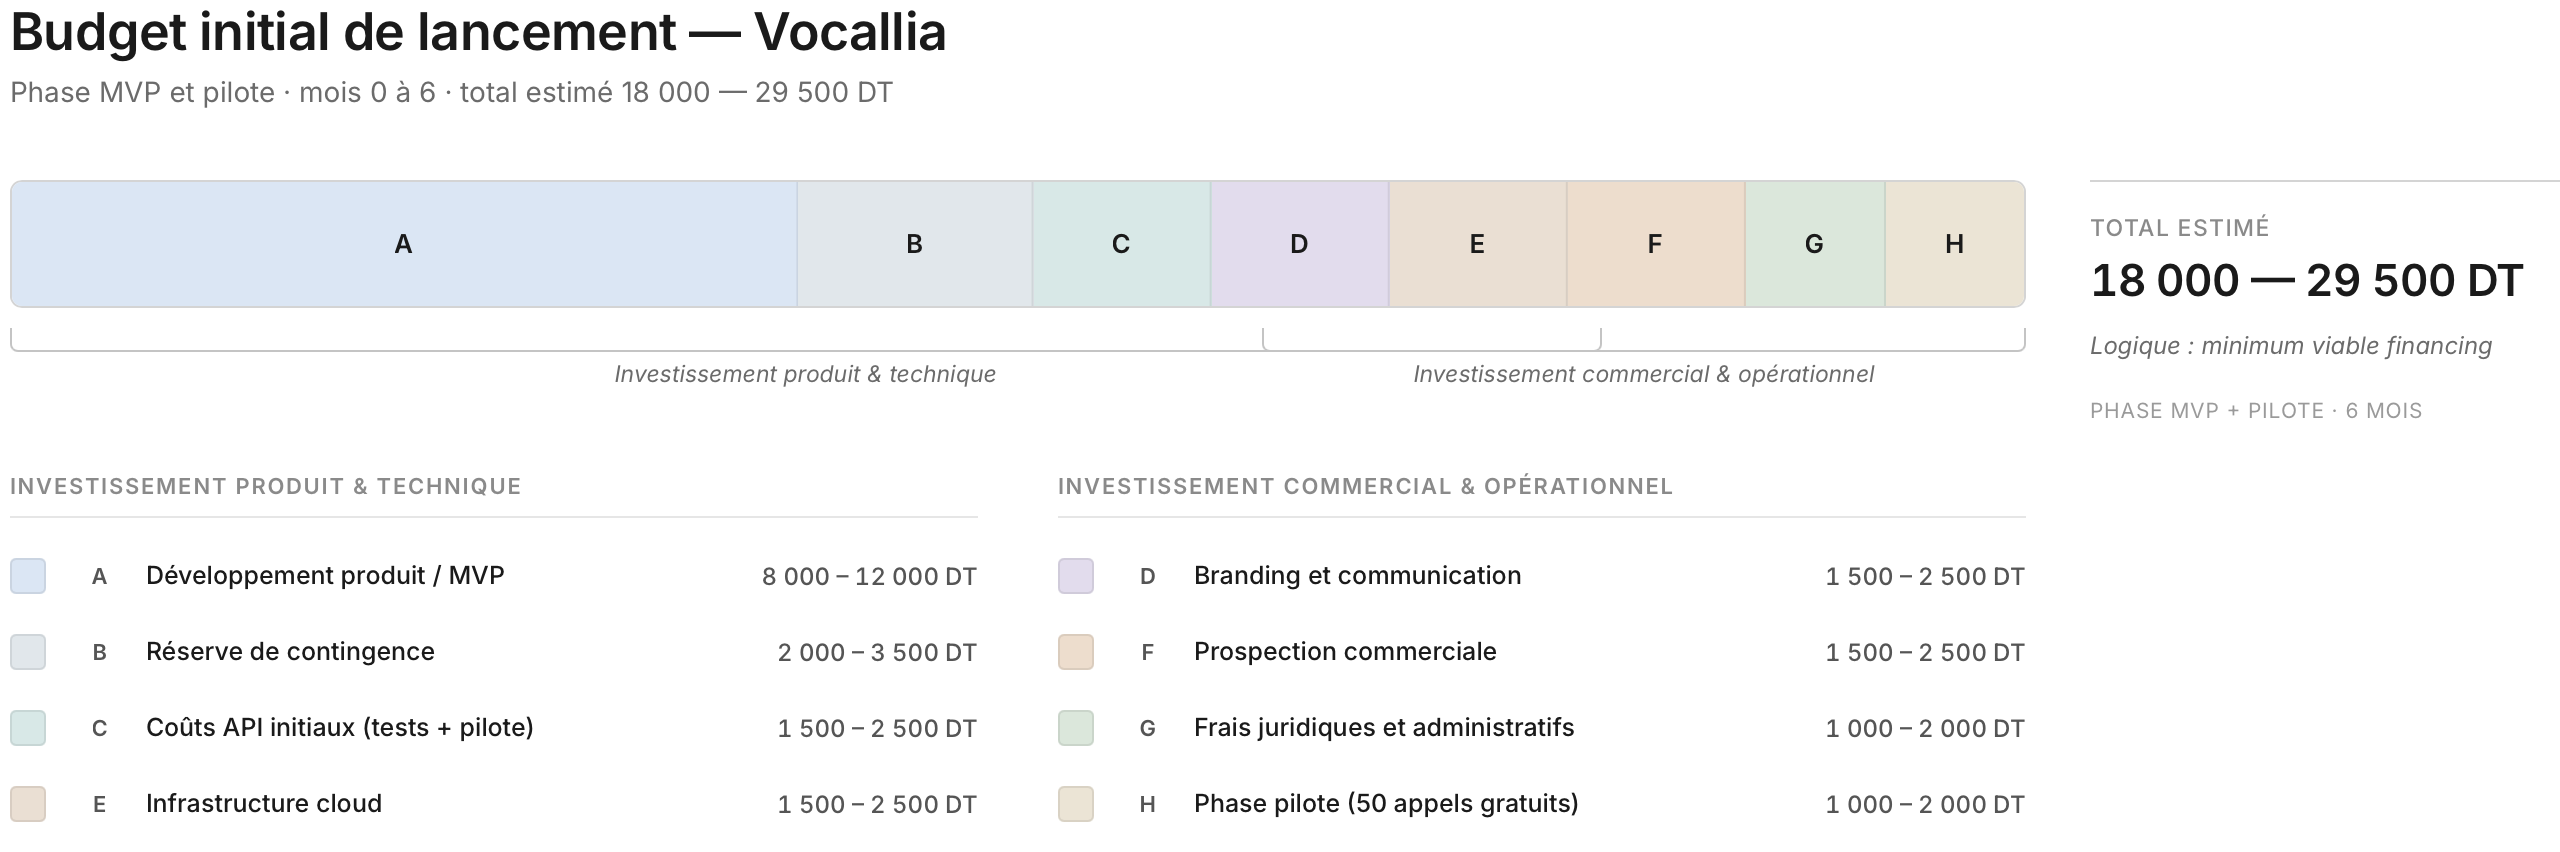
\includegraphics[width=\textwidth]{figures/budget-initial-lancement-vocallia.png}
\caption{Budget initial de lancement — phase MVP et pilote (mois 0--6)}
\label{fig:budget_initial}
\end{figure}

\begin{table}[H]
\centering
\caption{Investissement initial estimé — phase MVP et pilote (mois 0 à 6)}
\label{tab:investissement_initial}
\begin{tabular}{|p{5cm}|p{3cm}|p{6cm}|}
\hline
\textbf{Poste} & \textbf{Budget (DT)} & \textbf{Nature et justification} \\
\hline
Développement produit / MVP & 8\,000 — 12\,000 & Construction du pipeline conversationnel, dashboard, intégrations Shopify / WooCommerce \\
\hline
Infrastructure cloud et configuration technique & 1\,500 — 2\,500 & Mise en place initiale (Docker, Kubernetes managé, base de données, monitoring) \\
\hline
Coûts API initiaux (tests, calibrage, pilote) & 1\,500 — 2\,500 & STT, LLM, TTS et téléphonie sur volume de tests et premiers appels pilotes \\
\hline
Frais juridiques et administratifs & 1\,000 — 2\,000 & Constitution juridique, labellisation Startup Act, démarche INPDP préliminaire \\
\hline
Branding et communication & 1\,500 — 2\,500 & Identité visuelle, site web, landing page, vidéos de démonstration \\
\hline
Prospection commerciale initiale & 1\,500 — 2\,500 & Campagnes Meta Ads, outils CRM, déplacements, démonstrations directes \\
\hline
Phase pilote (50 appels gratuits par marchand) & 1\,000 — 2\,000 & Coût opérationnel des pilotes offerts (Product-Led Growth) \\
\hline
Réserve de contingence (10—15~\%) & 2\,000 — 3\,500 & Couverture des aléas techniques, juridiques et commerciaux \\
\hline
\textbf{Total estimé} & \textbf{18\,000 — 29\,500} & Budget de lancement minimum viable \\
\hline
\end{tabular}
\end{table}

\paragraph{Lecture stratégique.} Trois caractéristiques rendent cet investissement défendable. D'abord, une part significative du coût (développement produit) peut être valorisée comme contribution en nature des fondateurs, ce qui réduit le besoin de cash externe immédiat. Ensuite, le budget de prospection est calibré sur des canaux à coût marginal observé en phase exploratoire — la phase Muvaka d'avril 2025 ayant produit un coût par lead (CPL) de l'ordre de 0{,}36~euro, indicateur de \emph{génération de leads} et non de coût d'acquisition client confirmé, qui devra être validé une fois le premier cycle de conversion mesuré. Enfin, la réserve de contingence de l'ordre de 10 à 15~\% protège contre les aléas sans gonfler artificiellement le besoin de financement initial.

%%%%%%%%%%%%%%%%%%%%%%%%%%%%%%%%%%%%%%%%%%%%%%%%%%%%%%%%%%%%%%%%%%%%%%%%%%%
\section{Charges d'exploitation et structure de coûts}
\label{sec:charges_exploitation}
%%%%%%%%%%%%%%%%%%%%%%%%%%%%%%%%%%%%%%%%%%%%%%%%%%%%%%%%%%%%%%%%%%%%%%%%%%%

La structure de coûts de Vocallia présente une caractéristique stratégique majeure~: elle est \textbf{dominée par les coûts variables}, indexés sur le volume d'appels traités. Cette propriété, déjà soulignée au chapitre~3, est la condition mathématique de la scalabilité du modèle~: chaque client supplémentaire peut être servi sans déclencher de saut significatif de coûts fixes, sous réserve que la hausse soit absorbée par les capacités existantes de l'équipe. La figure~\ref{fig:structure_charges} en visualise la répartition.

\begin{figure}[H]
\centering
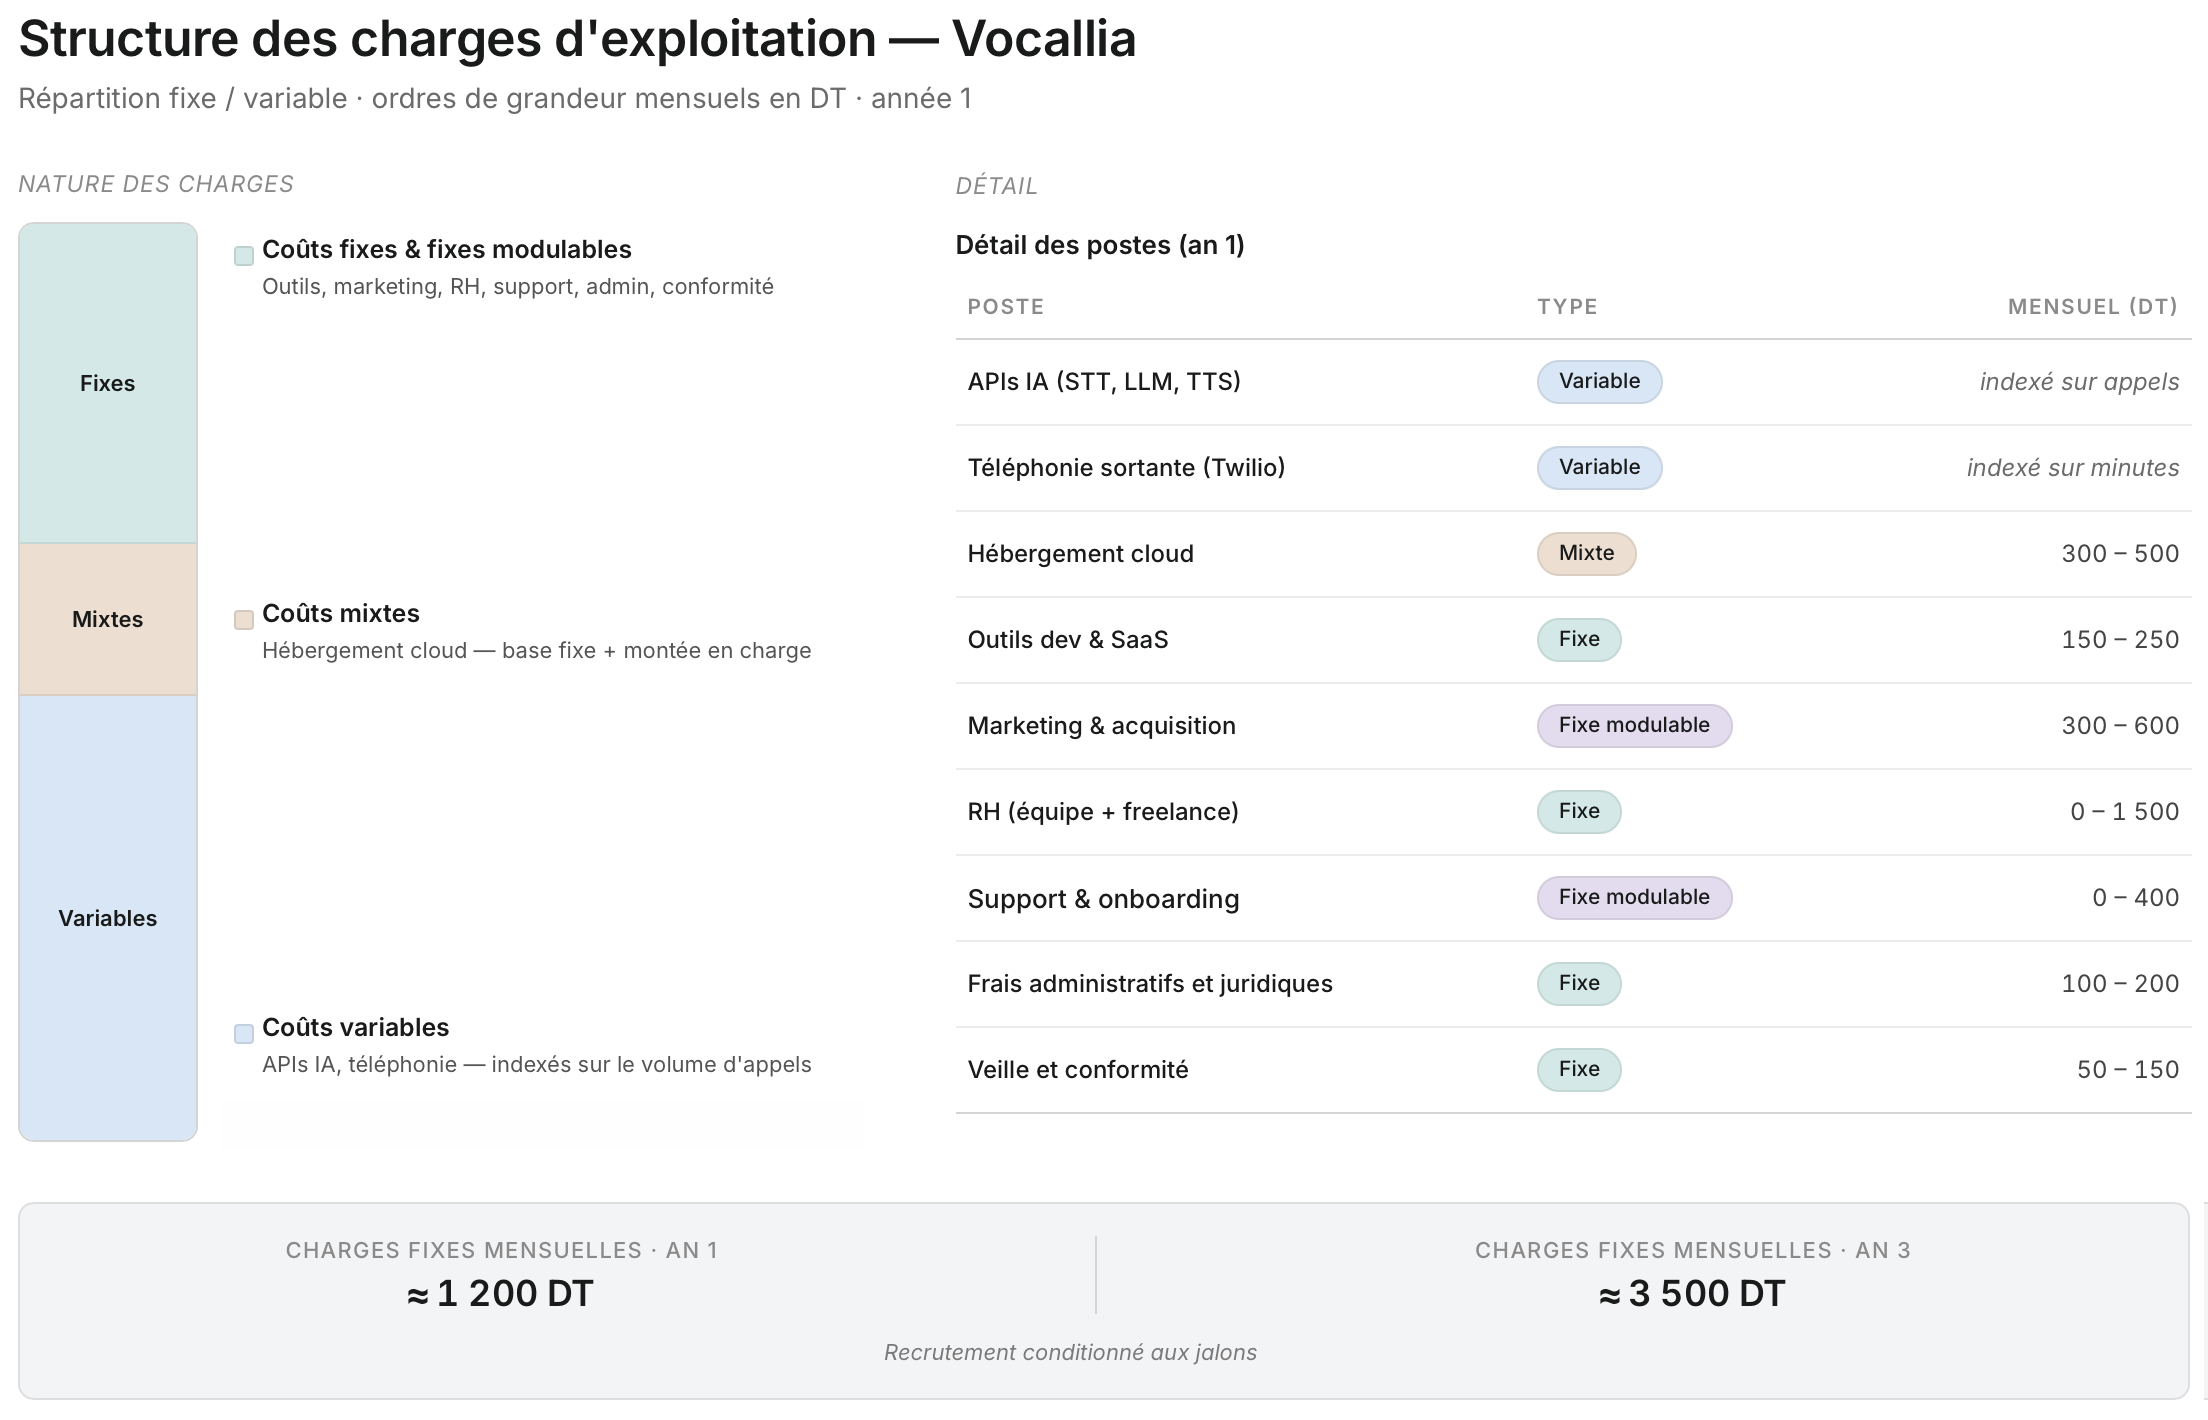
\includegraphics[width=\textwidth]{figures/structure-charges-exploitation-vocallia.png}
\caption{Structure des charges d'exploitation de Vocallia — répartition fixe / variable}
\label{fig:structure_charges}
\end{figure}

\begin{table}[H]
\centering
\caption{Structure des charges d'exploitation — Vocallia (en DT)}
\label{tab:charges_exploitation}
\begin{tabular}{|p{4cm}|p{2.5cm}|p{4cm}|p{4cm}|}
\hline
\textbf{Poste} & \textbf{Type} & \textbf{Ordre de grandeur mensuel (an~1)} & \textbf{Évolution attendue} \\
\hline
APIs IA (STT, LLM, TTS) & Variable & Indexé sur appels & Croît avec le volume, marge stable \\
\hline
Téléphonie sortante (Twilio) & Variable & Indexé sur minutes & Idem, négociable à l'échelle \\
\hline
Hébergement cloud (compute, stockage) & Mixte & 300 — 500 & Faible élasticité avant 200+ clients \\
\hline
Outils de développement et SaaS internes & Fixe & 150 — 250 & Stable \\
\hline
Marketing et acquisition (Meta Ads, SEO) & Fixe modulable & 300 — 600 & Augmente progressivement \\
\hline
Ressources humaines (équipe fondatrice + freelance) & Fixe & 0 — 1\,500 & Croissance conditionnée aux jalons \\
\hline
Support client et onboarding & Fixe modulable & 0 — 400 & À partir du mois~3 \\
\hline
Frais administratifs et juridiques & Fixe & 100 — 200 & Stable \\
\hline
Veille et conformité (INPDP, sécurité) & Fixe & 50 — 150 & Léger renforcement an~2 \\
\hline
\end{tabular}
\end{table}

\paragraph{Analyse de la structure.} Trois constats s'imposent. Les charges fixes mensuelles d'année~1 sont \textbf{volontairement contenues autour de 1\,200~DT}, niveau atteignable grâce à une équipe initiale réduite et à l'absence de loyer commercial. La part variable du coût total est \textbf{absorbée par la marge brute structurellement élevée} du plan Starter (de l'ordre de 65~\%, cf. chapitre~4)~: chaque appel facturé couvre largement son coût marginal. La hausse projetée des charges fixes en année~3 (vers 3\,500~DT/mois) est calibrée pour permettre un premier recrutement (commercial ou customer success) une fois le seuil de rentabilité opérationnel franchi — et non l'inverse. Cette discipline d'embauche conditionnée aux revenus est l'élément le plus important de la soutenabilité financière du modèle.

%%%%%%%%%%%%%%%%%%%%%%%%%%%%%%%%%%%%%%%%%%%%%%%%%%%%%%%%%%%%%%%%%%%%%%%%%%%
\section{Prévisions de chiffre d'affaires}
\label{sec:previsions_ca}
%%%%%%%%%%%%%%%%%%%%%%%%%%%%%%%%%%%%%%%%%%%%%%%%%%%%%%%%%%%%%%%%%%%%%%%%%%%

Le chiffre d'affaires de Vocallia est construit comme la somme de trois flux~: les abonnements mensuels récurrents (MRR), la facturation à l'usage des appels au-delà du forfait, et les frais ponctuels d'onboarding pour le palier Pro. Pour la projection, ces flux sont consolidés via un \textbf{ARPU pondéré} de l'ordre de 120~DT/mois, valeur cohérente avec un mix de portefeuille progressif Starter~$\to$~Croissance. La trajectoire du nombre de clients actifs prolonge directement les projections présentées au chapitre~3, en intégrant l'effet du churn mensuel et le rythme d'acquisition net.

\begin{table}[H]
\centering
\caption{Prévisions de chiffre d'affaires sur 3 ans — trois scénarios}
\label{tab:previsions_ca}
\begin{tabular}{|p{4cm}|p{3cm}|p{3cm}|p{3cm}|}
\hline
\textbf{Indicateur} & \textbf{Prudent} & \textbf{Central} & \textbf{Ambitieux} \\
\hline
\multicolumn{4}{|c|}{\textit{Année 1}} \\
\hline
Clients actifs (fin) & 20 & 40 & 65 \\
\hline
MRR fin d'année (DT) & $\sim$2\,400 & $\sim$4\,800 & $\sim$7\,800 \\
\hline
CA annuel (DT) & $\sim$22\,000 & $\sim$45\,000 & $\sim$72\,000 \\
\hline
\multicolumn{4}{|c|}{\textit{Année 2}} \\
\hline
Clients actifs (fin) & 35 & 70 & 120 \\
\hline
MRR fin d'année (DT) & $\sim$4\,200 & $\sim$8\,400 & $\sim$14\,400 \\
\hline
CA annuel (DT) & $\sim$40\,000 & $\sim$80\,000 & $\sim$140\,000 \\
\hline
\multicolumn{4}{|c|}{\textit{Année 3}} \\
\hline
Clients actifs (fin) & 50 & 100 & 180 \\
\hline
MRR fin d'année (DT) & $\sim$6\,000 & $\sim$12\,000 & $\sim$21\,600 \\
\hline
CA annuel (DT) & $\sim$60\,000 & $\sim$120\,000 & $\sim$220\,000 \\
\hline
\end{tabular}
\end{table}

\paragraph{Synthèse.} Ces projections sont délibérément conservatrices~: même le scénario ambitieux ne suppose qu'environ 5 nouveaux clients nets par mois en année~3, soit une dynamique modérée au regard de ce qui est généralement observé pour les SaaS B2B ayant atteint la traction \emph{product-market fit}. Le scénario prudent, lui, est calibré pour que le projet reste vivant même dans une configuration de croissance lente — propriété essentielle pour une thèse d'investissement défendable. Ces trajectoires restent toutefois des projections~: elles seront recalibrées à la lumière des données réelles d'acquisition et de churn observées en phase pilote.

%%%%%%%%%%%%%%%%%%%%%%%%%%%%%%%%%%%%%%%%%%%%%%%%%%%%%%%%%%%%%%%%%%%%%%%%%%%
\section{Compte de résultat prévisionnel}
\label{sec:compte_resultat}
%%%%%%%%%%%%%%%%%%%%%%%%%%%%%%%%%%%%%%%%%%%%%%%%%%%%%%%%%%%%%%%%%%%%%%%%%%%

Le compte de résultat prévisionnel agrège les hypothèses de revenus et de charges précédentes pour produire une estimation lisible de la marge brute et du résultat opérationnel sur 36~mois. Il est présenté ici dans le scénario central, considéré comme le plus probable. La figure~\ref{fig:projection_36_mois} en représente la trajectoire visuelle~: revenus, coûts variables, charges fixes et résultat opérationnel sur l'horizon complet de projection.

\begin{figure}[H]
\centering
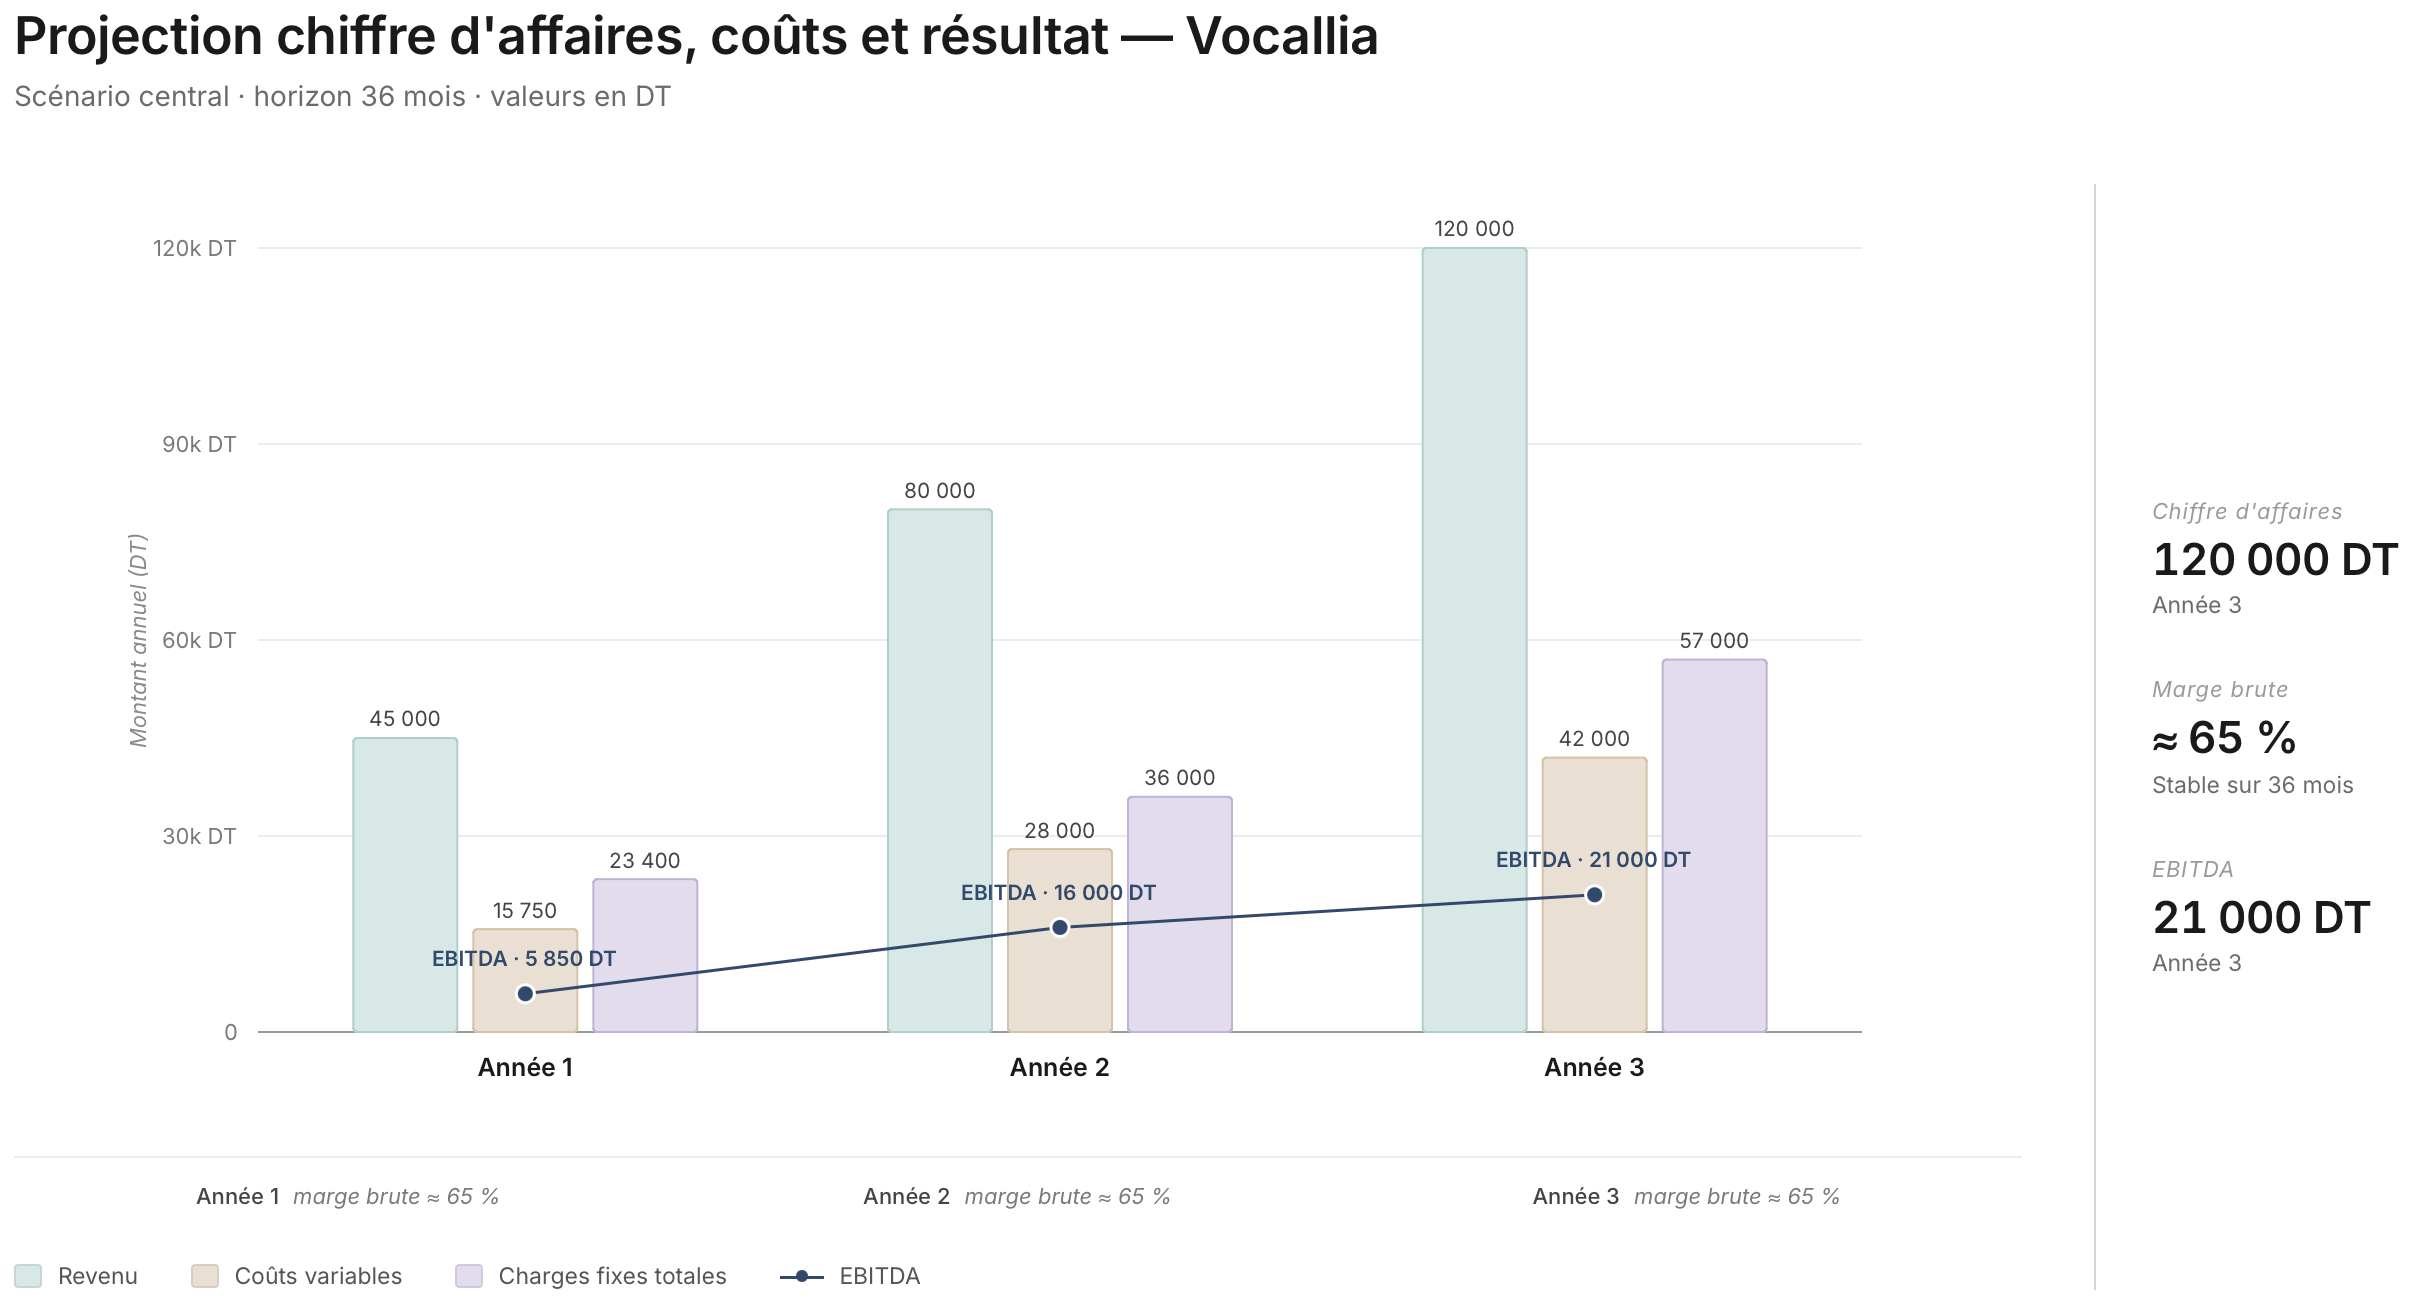
\includegraphics[width=\textwidth]{figures/projection-ca-couts-resultat-36-mois.png}
\caption{Projection chiffre d'affaires, coûts et résultat opérationnel sur 36 mois — scénario central}
\label{fig:projection_36_mois}
\end{figure}

\begin{table}[H]
\centering
\caption{Compte de résultat prévisionnel — scénario central (en DT)}
\label{tab:compte_resultat}
\begin{tabular}{|p{5cm}|p{3cm}|p{3cm}|p{3cm}|}
\hline
\textbf{Poste} & \textbf{Année 1} & \textbf{Année 2} & \textbf{Année 3} \\
\hline
Chiffre d'affaires & $\sim$45\,000 & $\sim$80\,000 & $\sim$120\,000 \\
\hline
Coûts variables (APIs, téléphonie, hébergement marginal) & $\sim$15\,750 & $\sim$28\,000 & $\sim$42\,000 \\
\hline
\textbf{Marge brute} & $\sim$29\,250 & $\sim$52\,000 & $\sim$78\,000 \\
\hline
Charges fixes opérationnelles & $\sim$14\,400 & $\sim$24\,000 & $\sim$42\,000 \\
\hline
Charges marketing et acquisition & $\sim$6\,000 & $\sim$8\,000 & $\sim$10\,000 \\
\hline
Charges administratives et conformité & $\sim$3\,000 & $\sim$4\,000 & $\sim$5\,000 \\
\hline
\textbf{Résultat opérationnel (EBITDA)} & $\sim$\,5\,850 & $\sim$16\,000 & $\sim$21\,000 \\
\hline
Amortissement de l'investissement initial & $\sim$6\,000 & $\sim$6\,000 & $\sim$6\,000 \\
\hline
\textbf{Résultat avant impôt} & $\sim$\,-150 & $\sim$10\,000 & $\sim$15\,000 \\
\hline
Impôts (régime Startup Act) & 0 — exonéré & 0 — exonéré & 0 — exonéré \\
\hline
\textbf{Résultat net estimé} & $\sim$\,-150 & $\sim$10\,000 & $\sim$15\,000 \\
\hline
\end{tabular}
\end{table}

\paragraph{Lecture analytique.} Le scénario central fait apparaître trois enseignements, qu'il convient de présenter avec prudence. D'abord, une marge brute structurellement élevée, qui reflète la dominance des coûts variables et la soutenabilité économique du palier Starter démontrée au chapitre~4. Ensuite, un \textbf{EBITDA légèrement positif dès la première année dans le scénario central}, soutenu par la modération volontaire des charges fixes — résultat conditionné au respect strict de la trajectoire d'acquisition et à la maîtrise des charges fixes. Enfin, un résultat net proche de l'équilibre en année~1 puis modérément positif en années~2 et~3, sous réserve que la trajectoire d'acquisition projetée soit effectivement tenue. En scénario prudent, le résultat net resterait négatif en années~1 et~2 et tendrait vers l'équilibre en année~3~; en scénario ambitieux, l'équilibre serait atteint plus tôt. Ces estimations doivent être lues comme des ordres de grandeur et non comme des engagements de performance.

%%%%%%%%%%%%%%%%%%%%%%%%%%%%%%%%%%%%%%%%%%%%%%%%%%%%%%%%%%%%%%%%%%%%%%%%%%%
\section{Seuil de rentabilité et analyse du point mort}
\label{sec:seuil_rentabilite}
%%%%%%%%%%%%%%%%%%%%%%%%%%%%%%%%%%%%%%%%%%%%%%%%%%%%%%%%%%%%%%%%%%%%%%%%%%%

\subsection{Méthodologie et calcul du point mort}
\label{subsec:methodo_seuil}

Le seuil de rentabilité opérationnel est défini comme le niveau de chiffre d'affaires — et donc de clients actifs — à partir duquel la marge brute couvre intégralement les charges fixes opérationnelles. Avec un ARPU pondéré d'environ 120~DT/mois et une marge brute de l'ordre de 65~\%, chaque client actif contribue à hauteur d'environ \textbf{78~DT/mois} à la couverture des charges fixes. Il s'agit ici d'un seuil de rentabilité \emph{opérationnel}, hors amortissement de l'investissement initial.

En appliquant cette contribution unitaire aux charges fixes mensuelles projetées, on obtient les seuils synthétisés dans le tableau~\ref{tab:seuil_rentabilite}, dont la figure~\ref{fig:seuil_rentabilite} fournit la lecture visuelle.

\begin{table}[H]
\centering
\caption{Seuil de rentabilité opérationnelle — Vocallia}
\label{tab:seuil_rentabilite}
\begin{tabular}{|p{3cm}|p{3.5cm}|p{4cm}|p{3.5cm}|}
\hline
\textbf{Année} & \textbf{Charges fixes mensuelles (DT)} & \textbf{Contribution par client (DT/mois)} & \textbf{Clients actifs au point mort} \\
\hline
Année 1 & $\sim$1\,200 & $\sim$78 & $\sim$15 — 16 \\
\hline
Année 2 & $\sim$2\,000 & $\sim$78 & $\sim$25 — 27 \\
\hline
Année 3 & $\sim$3\,500 & $\sim$78 & $\sim$45 \\
\hline
\end{tabular}
\end{table}

\begin{figure}[H]
\centering
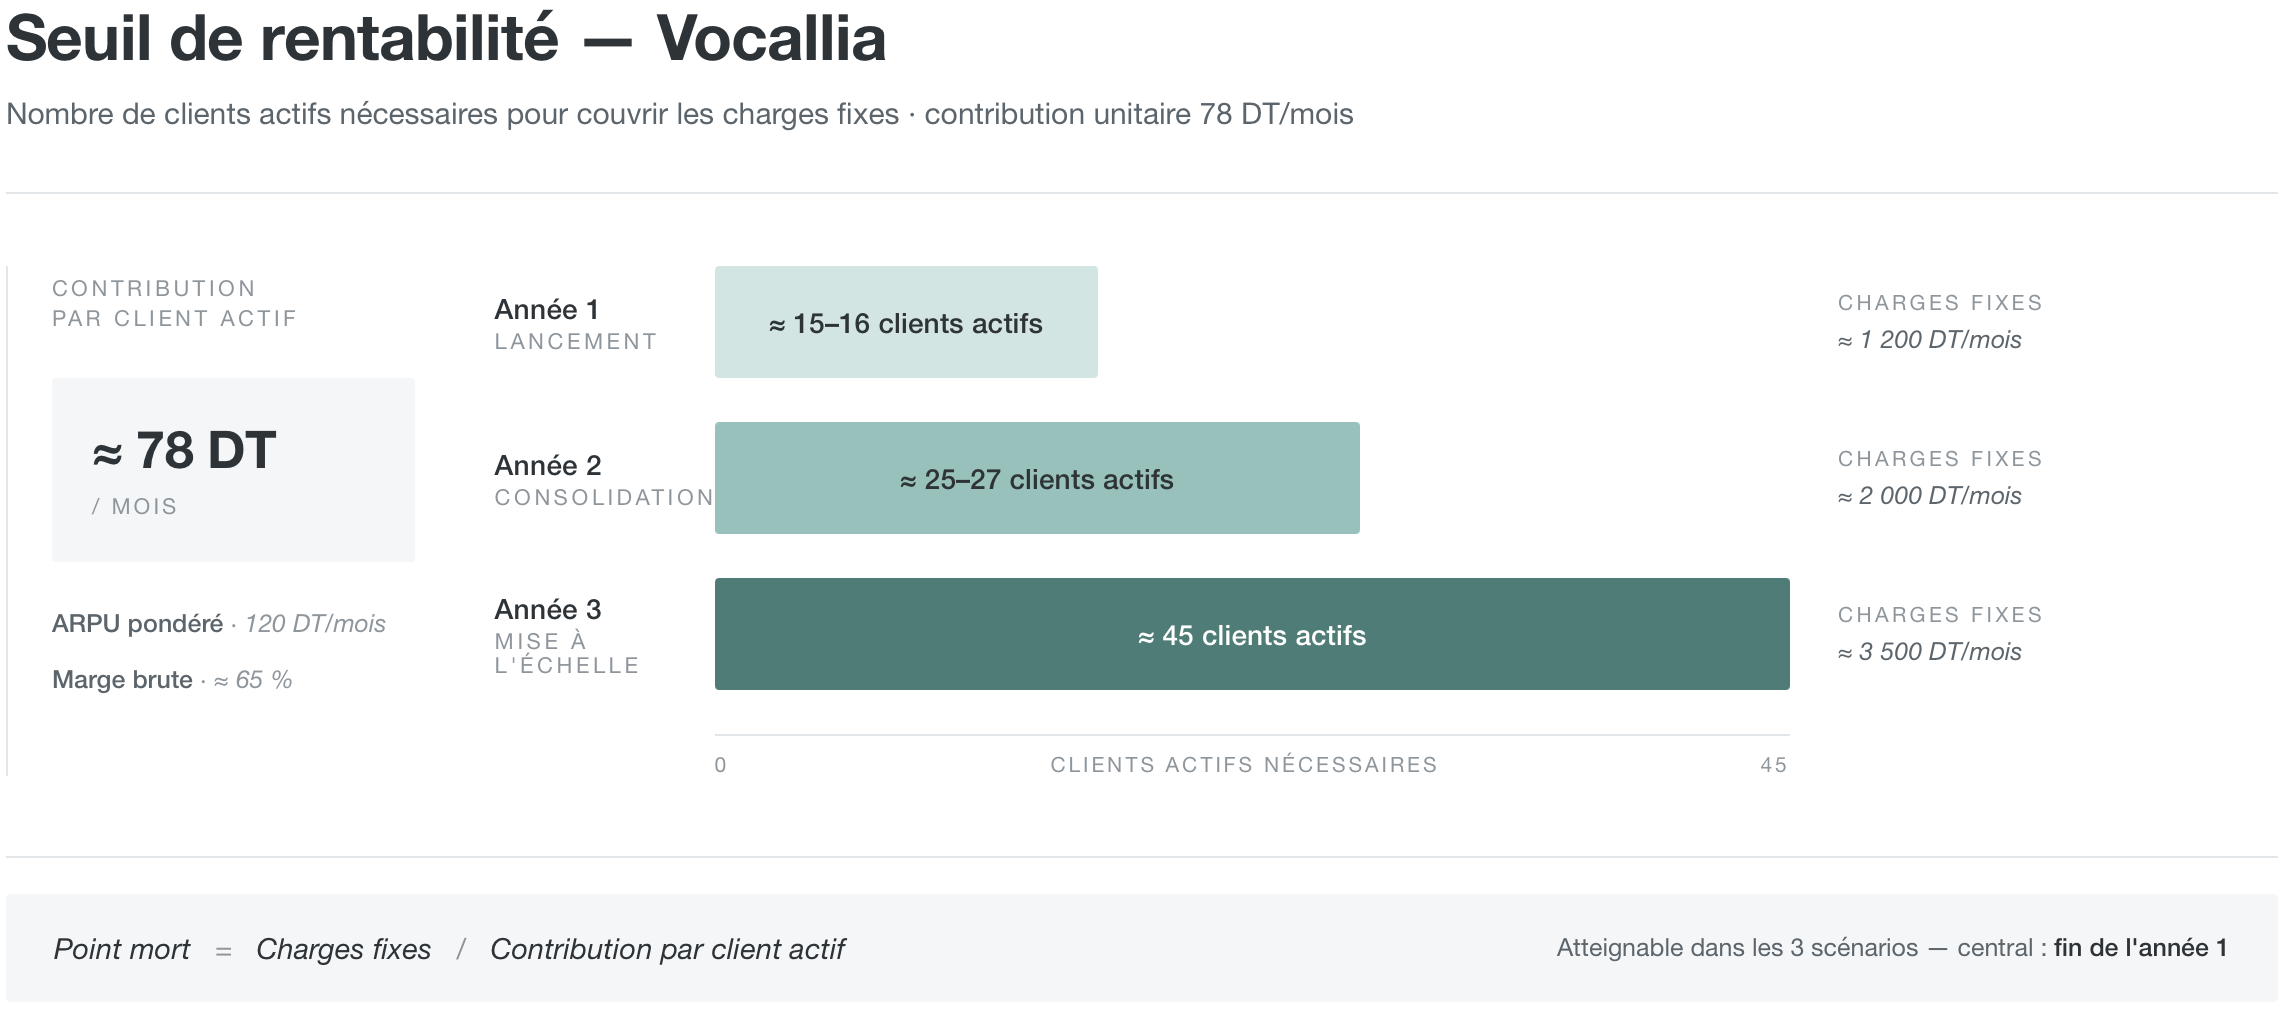
\includegraphics[width=\textwidth]{figures/seuil-rentabilite-clients-actifs.png}
\caption{Seuil de rentabilité — clients actifs nécessaires par année}
\label{fig:seuil_rentabilite}
\end{figure}

\begin{quote}
\textbf{Lecture stratégique.} Le seuil opérationnel apparaît atteignable dans tous les scénarios sous réserve de tenue de la trajectoire commerciale~: vers la fin du mois~12 dans le scénario central, plus tôt dans le scénario ambitieux, en cours d'année~3 dans le scénario prudent. Cette propriété est précisément le résultat de la discipline d'architecture frugale du chapitre~4 et du modèle PLG du chapitre~3~: en limitant volontairement les charges fixes en phase d'amorçage, Vocallia rend son point mort opérationnel accessible avec un nombre de clients qui correspond à la borne basse crédible des projections commerciales. Il convient toutefois de rappeler que ce seuil ne couvre pas l'amortissement de l'investissement initial, qui exigera une période plus longue pour être pleinement absorbé.
\end{quote}

\subsection{Sensibilité du point mort}
\label{subsec:sensibilite_seuil}

Trois variables affectent directement la trajectoire du point mort. Une \textbf{hausse de 20~\%} des coûts API (volatilité tarifaire) réduirait la marge brute d'environ 6~points et augmenterait le seuil de quelques clients seulement — sensibilité faible. Une \textbf{augmentation de 50~\%} des charges fixes (par exemple un recrutement anticipé) repousserait le point mort de 7 à 8 clients — sensibilité moyenne. Un \textbf{churn dégradé à 10~\%/mois} éroderait la LTV et exigerait un rythme d'acquisition brut sensiblement supérieur pour maintenir le même nombre de clients actifs nets — sensibilité élevée. Le churn est donc le levier le plus critique~: c'est lui qui doit faire l'objet de la surveillance la plus attentive en phase d'exécution.

%%%%%%%%%%%%%%%%%%%%%%%%%%%%%%%%%%%%%%%%%%%%%%%%%%%%%%%%%%%%%%%%%%%%%%%%%%%
\section{Plan de financement}
\label{sec:plan_financement}
%%%%%%%%%%%%%%%%%%%%%%%%%%%%%%%%%%%%%%%%%%%%%%%%%%%%%%%%%%%%%%%%%%%%%%%%%%%

La philosophie de financement retenue est résolument \textbf{progressive et non dilutive en priorité}. Plutôt que de lever un capital important en phase prématurée — ce qui imposerait une dilution significative et une pression de croissance disproportionnée — Vocallia structure son financement en couches superposées, chacune activée lorsque la précédente est consommée et que les jalons associés sont franchis. La figure~\ref{fig:plan_financement} en illustre le séquencement.

\begin{figure}[H]
\centering
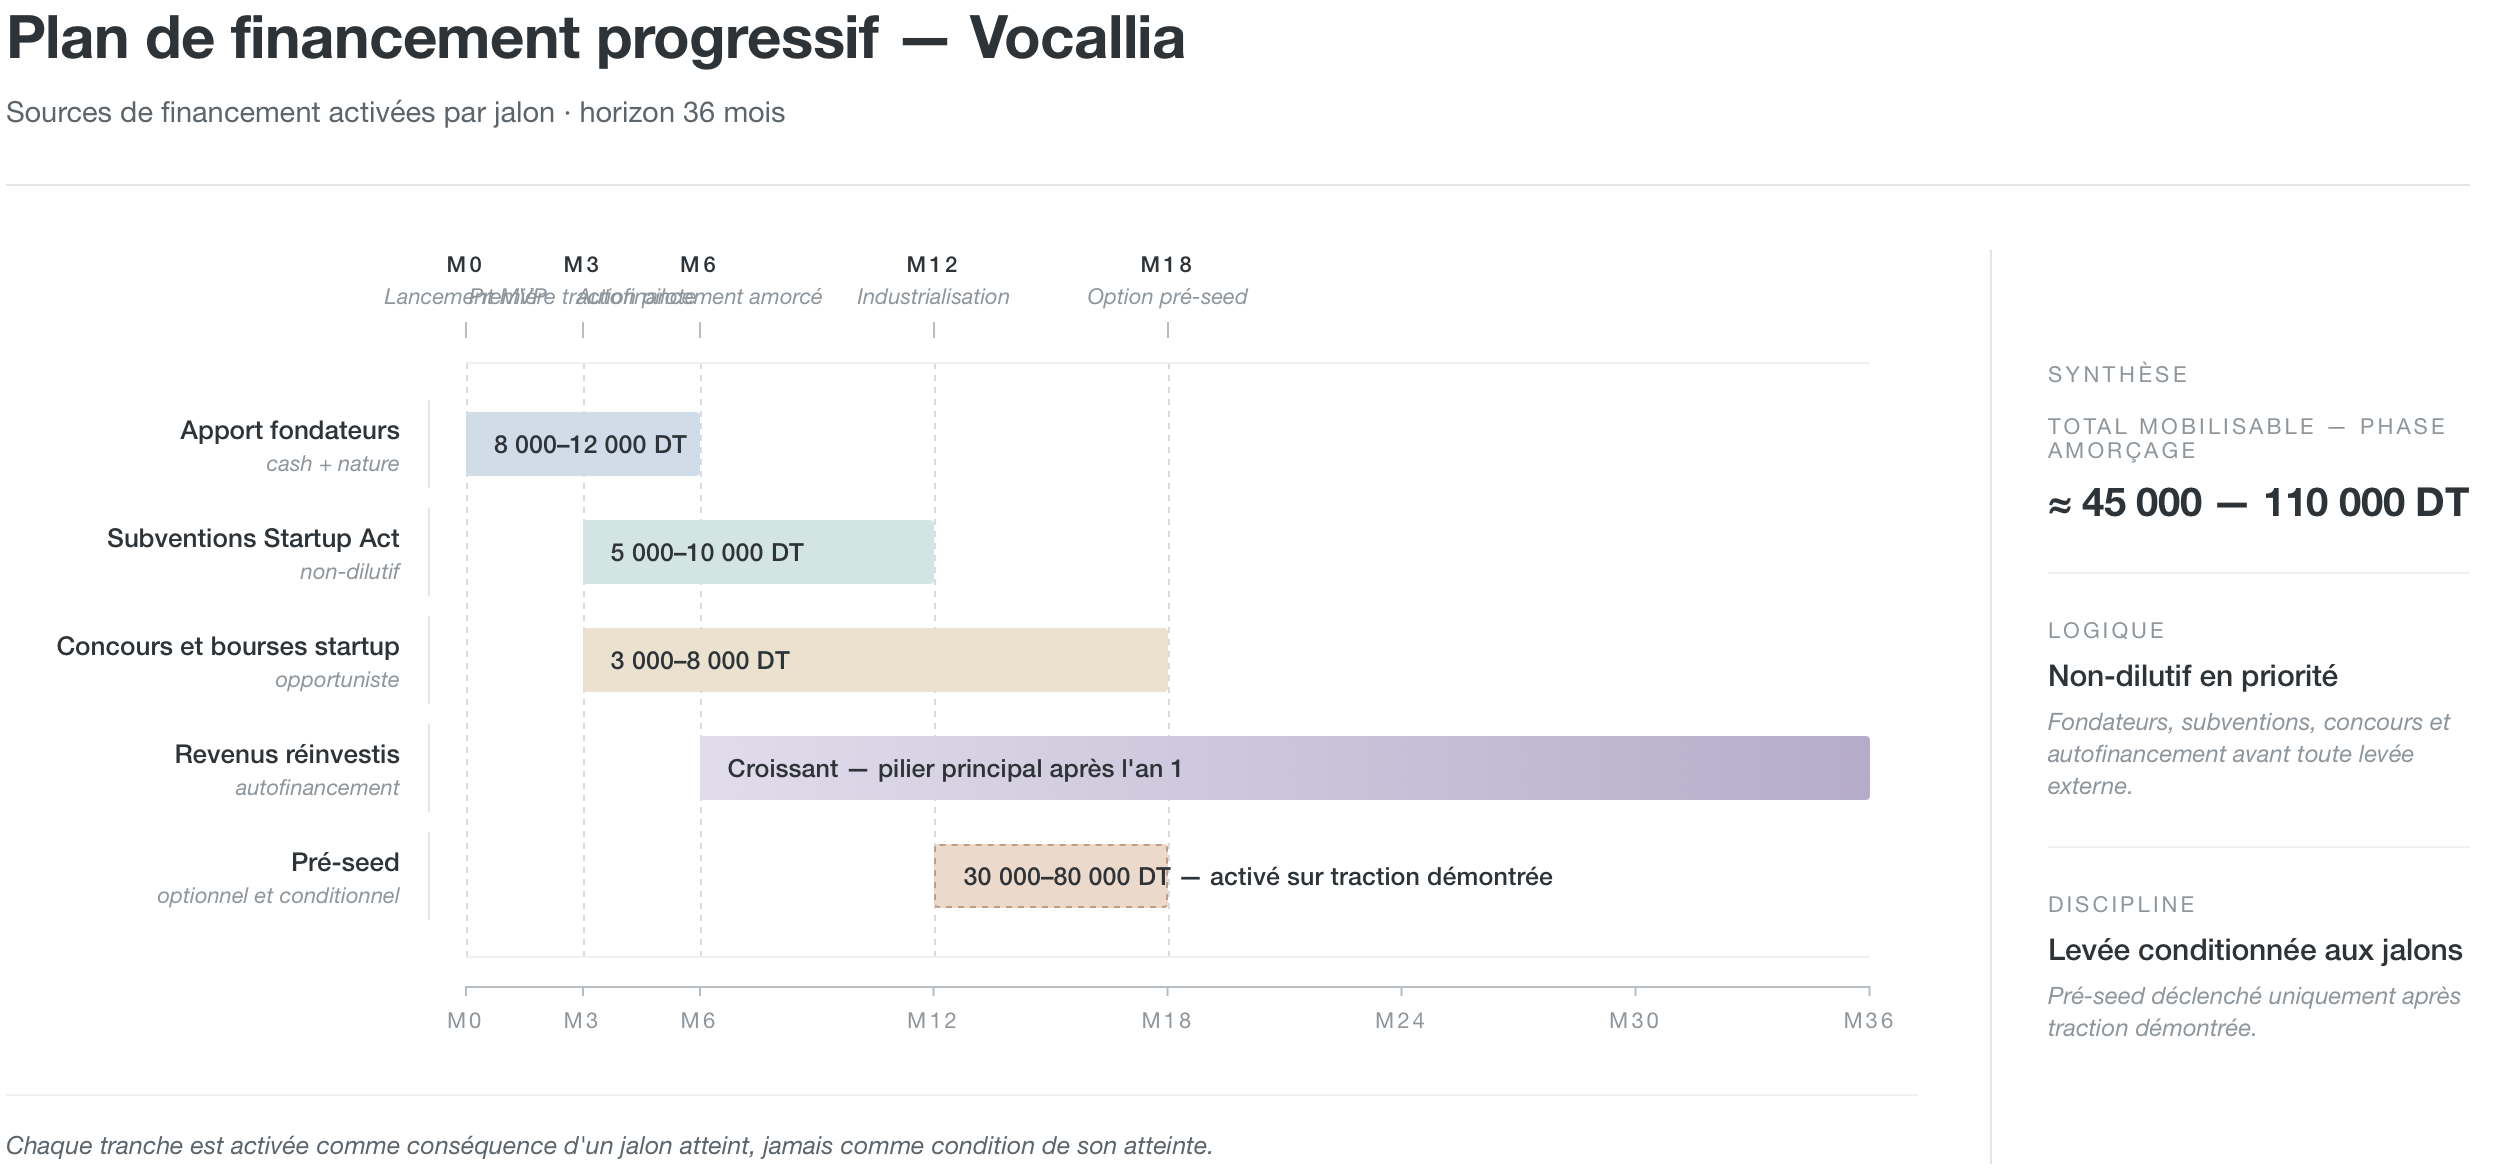
\includegraphics[width=\textwidth]{figures/plan-financement-progressif-vocallia.png}
\caption{Plan de financement progressif de Vocallia — sources et activation par jalon}
\label{fig:plan_financement}
\end{figure}

\begin{table}[H]
\centering
\caption{Plan de financement structuré — Vocallia (horizon 36 mois)}
\label{tab:plan_financement}
\begin{tabular}{|p{4cm}|p{3cm}|p{3cm}|p{4cm}|}
\hline
\textbf{Source} & \textbf{Montant cible (DT)} & \textbf{Horizon} & \textbf{Conditions / logique} \\
\hline
Apport fondateurs (cash + nature) & 8\,000 — 12\,000 & Mois~0 & Développement MVP, premiers tests \\
\hline
Subventions et appuis Startup Act & 5\,000 — 10\,000 & Mois~3 — Mois~12 & Labellisation, BFG, primes mensuelles \\
\hline
Concours et bourses startup & 3\,000 — 8\,000 & Mois~3 — Mois~18 & Conditionné à la traction démontrée \\
\hline
Revenus réinvestis (autofinancement) & Croissant & À partir du mois~6 & Pilier principal après l'an~1 \\
\hline
Pré-seed potentiel (optionnel) & 30\,000 — 80\,000 & Mois~12 — Mois~18 & Activé seulement si trajectoire ambitieuse \\
\hline
\textbf{Total mobilisable phase amorçage} & \textbf{$\sim$45\,000 — 110\,000} & — & Modulé selon scénario \\
\hline
\end{tabular}
\end{table}

\paragraph{Justification du séquençage.} Trois raisons fondent ce séquençage. Le \textbf{Startup Act} (loi n°2018-20) offre un dispositif particulièrement avantageux dont l'activation précoce — labellisation dès la phase MVP — peut débloquer exonérations fiscales, accès devises et primes mensuelles, sans dilution. Le modèle économique permet une \textbf{contribution progressive de l'autofinancement à partir du mois~6}, dans la mesure où la marge brute couvre déjà à ce stade une part des charges fixes~: chaque client actif réduit alors progressivement la dépendance aux financements externes pour les charges courantes. Le recours à un \textbf{tour pré-seed} n'est envisagé que de manière conditionnelle, lorsqu'une traction documentée (15 à 25 clients actifs payants, MRR autour de 3\,000~DT, churn maîtrisé) permet de négocier des conditions favorables — situation très différente d'une levée prématurée.

\begin{quote}
\textbf{Discipline de financement.} Lever trop tôt est l'un des risques les plus sous-estimés des startups SaaS d'amorçage~: cela impose des objectifs de croissance déconnectés des fondamentaux du produit. Vocallia inverse délibérément cette logique~: chaque tranche de financement est activée comme conséquence d'un jalon atteint, et non comme condition préalable de son atteinte.
\end{quote}

%%%%%%%%%%%%%%%%%%%%%%%%%%%%%%%%%%%%%%%%%%%%%%%%%%%%%%%%%%%%%%%%%%%%%%%%%%%
\section{Indicateurs de rentabilité}
\label{sec:indicateurs_rentabilite}
%%%%%%%%%%%%%%%%%%%%%%%%%%%%%%%%%%%%%%%%%%%%%%%%%%%%%%%%%%%%%%%%%%%%%%%%%%%

\subsection{Approche méthodologique et précautions}
\label{subsec:methodo_indicateurs}

Calculer une VAN ou un TRI rigoureux à ce stade exigerait des hypothèses précises sur le taux d'actualisation, la structure de capital, la valeur terminale et la durée d'extrapolation, dont aucune n'est aujourd'hui suffisamment stabilisée pour produire un chiffre défendable au centième près. Plutôt que d'inventer une fausse précision, ce chapitre présente un \textbf{cadre indicatif} fondé sur les flux du scénario central, en identifiant clairement les paramètres qui devront être affinés à l'issue de la phase pilote.

\subsection{Indicateurs estimés}
\label{subsec:indicateurs_estimes}

\paragraph{Période de retour estimée de l'investissement initial.} Avec un investissement initial estimé autour de 25\,000~DT et un EBITDA cumulé estimé d'environ 42\,000~DT sur 3~ans en scénario central, l'investissement initial pourrait, en première approche, être absorbé entre la fin de l'année~2 et le milieu de l'année~3, soit une période de retour indicative \textbf{de l'ordre de 24 à 30 mois}. Cette estimation suppose toutefois que l'EBITDA généré soit intégralement disponible pour absorber l'investissement initial, ce qui ne tient pas compte d'éventuels besoins en fonds de roulement ou réinvestissements produit qui pourraient l'allonger. Cette durée reste néanmoins cohérente avec ce qui est généralement attendu sur les SaaS B2B en phase d'amorçage.

\paragraph{Cash-flow opérationnel et cash-flow cumulé.} Il convient de distinguer deux notions souvent confondues. Le \textbf{cash-flow opérationnel} (généré par l'exploitation courante hors investissement initial) pourrait devenir légèrement positif dès la fin de l'année~1 dans le scénario central, dans la continuité du résultat opérationnel projeté. Le \textbf{cash-flow cumulé} (intégrant l'investissement initial de l'ordre de 25\,000~DT) resterait en revanche négatif sur la majeure partie de l'horizon~: il devrait progressivement converger vers l'équilibre au cours de l'année~2 dans le scénario central, et n'atteindrait une trajectoire franchement positive qu'en année~3. En scénario prudent, le cash-flow cumulé resterait négatif plus longtemps, ce qui justifie la mobilisation des subventions et concours en complément.

\paragraph{LTV/CAC et CAC payback — cadre indicatif.} Comme indiqué au chapitre~3, le ratio LTV/CAC visé se situe au-dessus du seuil minimal de 3~:~1 généralement attendu par les investisseurs SaaS, et le CAC payback est ciblé en deçà de 6~mois. Ces ratios reposent toutefois sur des hypothèses de churn, d'ARPU et de coût d'acquisition qui devront être confirmées par les données réelles de la phase pilote. À ce stade, le CPL de l'ordre de 0{,}36~euro observé pendant la phase Muvaka constitue un signal favorable de génération de leads, mais ne préjuge pas du coût d'acquisition client effectif, qui dépendra du taux de conversion observé une fois le pilote engagé.

\paragraph{VAN et TRI — cadre indicatif.} À titre purement indicatif, et sous réserve de stabilisation des hypothèses, une projection à 5~ans avec un taux d'actualisation de l'ordre de 15~\% (cohérent avec un risque pays / risque early-stage en zone MENA) ferait apparaître une VAN potentiellement positive en scénario central, sous l'hypothèse explicite que la trajectoire d'acquisition soit prolongée au-delà de l'horizon de 36~mois et que les hypothèses de marge soient confirmées. Le TRI ne peut pas être chiffré de manière crédible avant l'achèvement de la phase pilote, qui fournira les données réelles d'acquisition, de churn et d'expansion nécessaires. Ces deux indicateurs doivent donc être présentés ici comme un \emph{cadre méthodologique}, et non comme des résultats de calcul.

%%%%%%%%%%%%%%%%%%%%%%%%%%%%%%%%%%%%%%%%%%%%%%%%%%%%%%%%%%%%%%%%%%%%%%%%%%%
\section{Plan d'exécution opérationnelle}
\label{sec:plan_execution}
%%%%%%%%%%%%%%%%%%%%%%%%%%%%%%%%%%%%%%%%%%%%%%%%%%%%%%%%%%%%%%%%%%%%%%%%%%%

Le plan d'exécution opérationnelle articule en quatre phases la transformation du projet en activité économique pérenne. Il croise quatre familles de jalons~: \textbf{technique} (cf.~chapitre~4), \textbf{commercial} (cf.~chapitre~3), \textbf{financier} (présent chapitre) et \textbf{réglementaire} (engagement INPDP, labellisation Startup Act). La figure~\ref{fig:roadmap_execution} en propose une représentation séquentielle.

\begin{figure}[H]
\centering
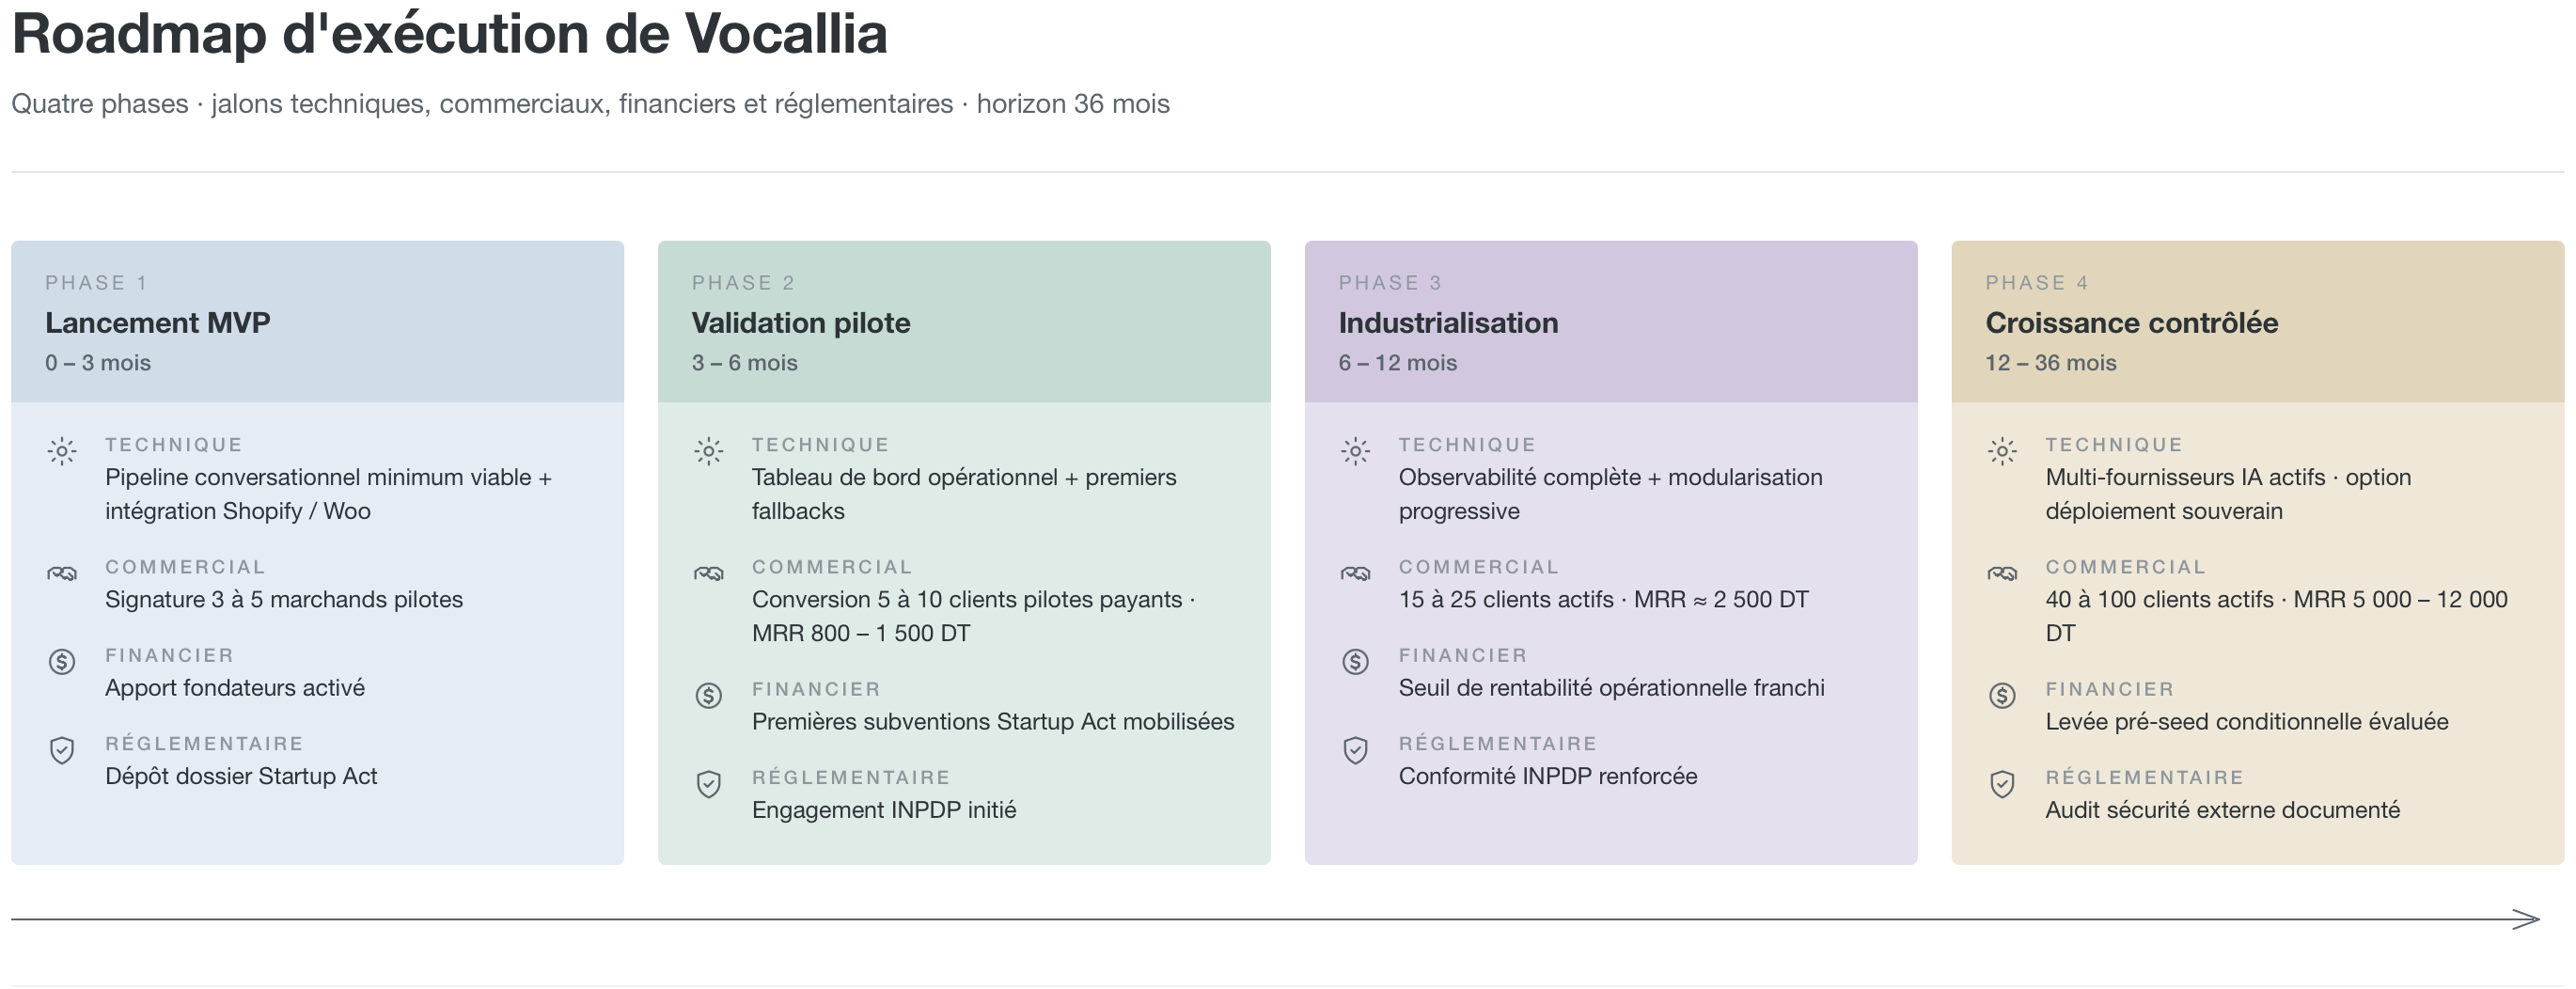
\includegraphics[width=\textwidth]{figures/roadmap-execution-vocallia.png}
\caption{Roadmap d'exécution de Vocallia — du MVP à la production (0--36 mois)}
\label{fig:roadmap_execution}
\end{figure}

\subsection{Phase 0--3 mois — Lancement du MVP}
\label{subsec:phase_0_3}

L'objectif est de mettre en service un MVP fonctionnel intégré à une plateforme e-commerce et utilisable par 1 à 3 marchands pilotes. Jalons critiques~: livraison du pipeline conversationnel minimum viable, mise en place du tableau de bord et des intégrations de base, dépôt du dossier Startup Act, lancement des premières campagnes Meta Ads, signature des 3 à 5 premiers pilotes.

\subsection{Phase 3--6 mois — Validation pilote}
\label{subsec:phase_3_6}

Le pilote vise à transformer les premiers utilisateurs gratuits en clients payants, en démontrant la valeur économique mesurable côté marchand. Jalons~: conversion de 5 à 10 clients pilotes en abonnements payants, atteinte d'un MRR de 800 à 1\,500~DT, premier rapport mensuel automatisé livré, engagement INPDP initié, premier témoignage client publié.

\subsection{Phase 6--12 mois — Industrialisation}
\label{subsec:phase_6_12}

L'objectif est de stabiliser le produit en production, viser le seuil de rentabilité opérationnelle et structurer les processus commerciaux et techniques. Jalons~: 15 à 25 clients actifs en scénario central, MRR autour de 2\,500~DT, mise en place de l'observabilité complète, modularisation progressive de l'architecture, premier recrutement freelance customer success conditionné au seuil franchi, lancement du programme de parrainage.

\subsection{Phase 12--36 mois — Croissance contrôlée}
\label{subsec:phase_12_36}

La trajectoire de moyen terme combine élargissement vertical (relance après abandon, prise de RDV, qualification de leads) et densification horizontale (acquisition de nouveaux marchands e-commerce). Jalons~: 40 à 100 clients actifs en scénario central, MRR entre 5\,000 et 12\,000~DT, premier recrutement permanent (commercial), évaluation conditionnelle d'une levée pré-seed, déploiement éventuel de l'option d'hébergement souverain pour comptes institutionnels.

\paragraph{Synthèse.} La séquence est calibrée pour que chaque investissement (recrutement, levée, expansion sectorielle) soit la \emph{conséquence} d'un jalon atteint, jamais sa \emph{condition} de financement. C'est précisément ce qui distingue un plan d'exécution discipliné d'un plan d'exécution optimiste.

%%%%%%%%%%%%%%%%%%%%%%%%%%%%%%%%%%%%%%%%%%%%%%%%%%%%%%%%%%%%%%%%%%%%%%%%%%%
\section{Impact économique et social}
\label{sec:impact_economique_social}
%%%%%%%%%%%%%%%%%%%%%%%%%%%%%%%%%%%%%%%%%%%%%%%%%%%%%%%%%%%%%%%%%%%%%%%%%%%

L'impact attendu de Vocallia dépasse la stricte performance financière de l'entreprise. Cinq dimensions méritent d'être explicitées, dans la continuité de l'analyse PESTEL conduite au chapitre~2.

\paragraph{Réduction des pertes pour l'écosystème e-commerce tunisien.} En contribuant à diminuer le taux de retours non anticipés et de ventes perdues faute de joignabilité, Vocallia peut produire un effet d'économie agrégée pour les marchands~: à l'échelle de quelques dizaines de PME équipées, les économies cumulées sur les coûts logistiques et le temps opérationnel libéré atteindraient des ordres de grandeur significatifs au regard de la taille du marché.

\paragraph{Gains de productivité et formalisation des opérations.} Pour le marchand, la confirmation automatisée pourrait libérer une part notable du temps gérant — capital humain réinjecté dans des tâches à plus forte valeur (croissance, achats, expérience client). Au-delà du gain individuel, le tableau de bord et les rapports mensuels participent d'une \textbf{formalisation progressive} des opérations e-commerce locales, contribution non négligeable à la professionnalisation du secteur.

\paragraph{Soutien à l'entrepreneuriat numérique tunisien.} Vocallia s'inscrit dans la dynamique du Startup Act et participe à l'émergence d'une nouvelle génération de startups SaaS tunisiennes développant des produits adaptés au contexte local — par opposition à une logique de simple intégration de solutions étrangères.

\paragraph{Création potentielle d'emplois qualifiés.} Au-delà du noyau fondateur, la trajectoire prévoit un premier recrutement en année~2 (customer success ou commercial), puis l'élargissement progressif de l'équipe, conditionné à l'atteinte des jalons financiers. L'écosystème d'intégrateurs, de consultants et de partenaires commerciaux pourrait également générer des opportunités indirectes.

\paragraph{Renforcement des capacités locales en IA appliquée.} Le corpus dialectal propriétaire que Vocallia construit progressivement constitue, à terme, un actif d'intérêt stratégique pour la communauté technologique locale~: il documente le darija dans un format exploitable par d'autres applications (santé, services publics, éducation) et représente un ancrage concret du développement de l'IA appliquée au contexte tunisien.

%%%%%%%%%%%%%%%%%%%%%%%%%%%%%%%%%%%%%%%%%%%%%%%%%%%%%%%%%%%%%%%%%%%%%%%%%%%
\section{Analyse des risques financiers et opérationnels}
\label{sec:risques_financiers}
%%%%%%%%%%%%%%%%%%%%%%%%%%%%%%%%%%%%%%%%%%%%%%%%%%%%%%%%%%%%%%%%%%%%%%%%%%%

Aucun plan financier ne tient sans une cartographie lucide de ses risques. Vocallia identifie huit risques principaux, classés selon leur probabilité et leur impact, et associe à chacun une mesure de mitigation directement opérationnelle. La figure~\ref{fig:matrice_risques} en propose une représentation matricielle.

\begin{figure}[H]
\centering
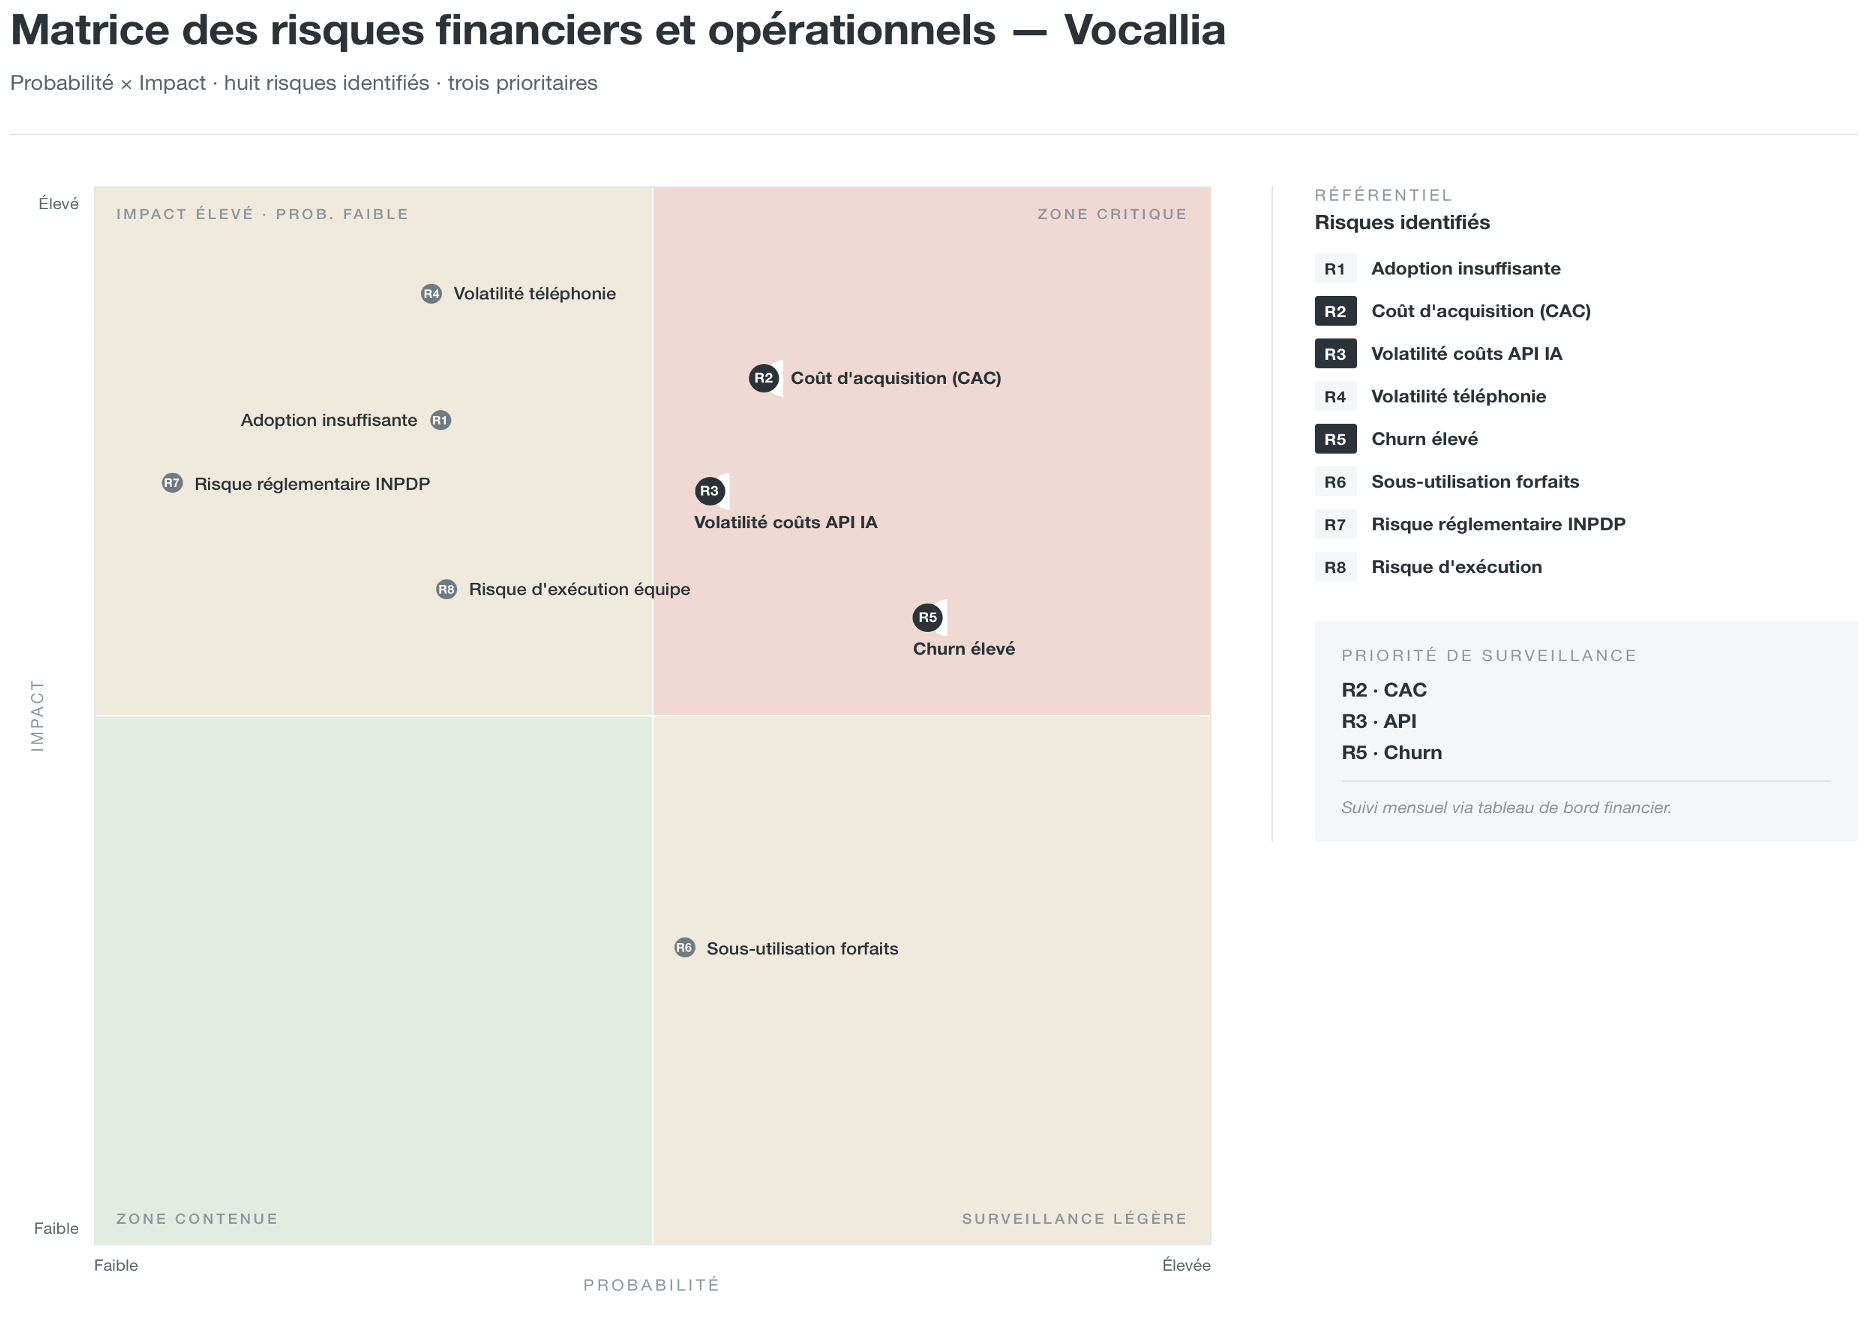
\includegraphics[width=\textwidth]{figures/matrice-risques-financiers-vocallia.png}
\caption{Matrice des risques financiers et opérationnels — Vocallia}
\label{fig:matrice_risques}
\end{figure}

\begin{table}[H]
\centering
\caption{Risques financiers et opérationnels — mesures de mitigation}
\label{tab:risques}
\begin{tabular}{|p{3.5cm}|p{4cm}|p{6cm}|}
\hline
\textbf{Risque} & \textbf{Nature et impact} & \textbf{Mesures de mitigation} \\
\hline
Adoption insuffisante & Rythme d'acquisition inférieur aux hypothèses, MRR sous-cible & Pilote gratuit, démonstration directe, programme de parrainage, focus Segment~A \\
\hline
Coût d'acquisition (CAC) dérapant & Dégradation du LTV/CAC, payback allongé & Suivi hebdomadaire du CPL, optimisation continue des campagnes Meta, canaux gratuits (SEO, bouche-à-oreille) \\
\hline
Volatilité des coûts API IA & Compression de la marge brute & Architecture multi-fournisseurs, veille tarifaire mensuelle, négociation à l'échelle dès an~2 \\
\hline
Volatilité des coûts de téléphonie & Idem, impact direct sur le coût par appel & Multi-opérateurs, partenariat futur potentiel avec opérateur local tunisien \\
\hline
Churn élevé & Dégradation de la LTV, point mort plus difficile à tenir & Onboarding renforcé, dashboard de valeur, rapport mensuel automatique, NPS suivi \\
\hline
Sous-utilisation des forfaits & Clients qui n'épuisent pas leurs appels inclus, frein à l'upgrade & Animation produit, suggestions automatiques d'extensions de cas d'usage \\
\hline
Risque réglementaire (INPDP) & Délais d'agrément, contraintes ajoutées en cours de route & Engagement proactif dès la phase pilote, conformité by design \\
\hline
Risque d'exécution (équipe restreinte) & Surcharge fondateurs, retards techniques ou commerciaux & Scoping strict du MVP, recours mesuré à freelances, recrutement conditionné aux jalons \\
\hline
\end{tabular}
\end{table}

\paragraph{Hiérarchisation des risques.} Trois risques se distinguent par leur probabilité et leur impact combinés~: le \textbf{churn}, le \textbf{coût d'acquisition} et la \textbf{volatilité des coûts API}. Ce sont eux qui doivent faire l'objet d'un suivi rapproché par un tableau de bord financier mensuel dès la phase pilote. Les autres risques sont structurellement contenus par les choix d'architecture et de gouvernance présentés dans les chapitres précédents, sans qu'aucun ne puisse être considéré comme totalement neutralisé.

%%%%%%%%%%%%%%%%%%%%%%%%%%%%%%%%%%%%%%%%%%%%%%%%%%%%%%%%%%%%%%%%%%%%%%%%%%%
\section{Conclusion}
\label{sec:conclusion_chap5}
%%%%%%%%%%%%%%%%%%%%%%%%%%%%%%%%%%%%%%%%%%%%%%%%%%%%%%%%%%%%%%%%%%%%%%%%%%%

L'analyse financière conduite dans ce chapitre établit quatre conclusions qui complètent et nuancent la démonstration de viabilité globale de Vocallia.

\textbf{Le modèle paraît financièrement viable, sous condition de discipline d'exécution.} La marge brute soutenable de l'ordre de 65~\% sur le palier Starter, combinée à une structure de coûts fixes volontairement contenue en phase d'amorçage, rend le seuil de rentabilité opérationnelle atteignable vers la fin de la première année dans le scénario central. Cette propriété n'est cependant pas automatique~: elle suppose le respect de la trajectoire d'acquisition et la maîtrise du churn, qui en constituent les deux conditions critiques.

\textbf{Le modèle paraît financièrement soutenable, à condition d'une adoption progressive et d'une exécution rigoureuse.} Le scénario prudent montre que même avec un rythme d'acquisition lent, le projet ne s'effondre pas~: il tend vers l'équilibre en année~3 plutôt qu'en année~1. Cette résilience financière distingue précisément un plan défendable d'un plan optimiste.

\textbf{Le modèle est structurellement scalable, parce que sa structure de coûts est dominée par les variables.} Chaque client supplémentaire améliore la marge sans déclencher de saut de coûts fixes immédiat. C'est la traduction financière directe de la modularité technique du chapitre~4 et de la stratégie PLG du chapitre~3.

\textbf{Le modèle est finançable de manière progressive, parce que l'investissement initial peut être étalé.} Le séquençage du financement — apport fondateurs, Startup Act, autofinancement progressif, levée conditionnelle — évite le piège de la sur-capitalisation prématurée et permet à chaque tranche de financement d'être justifiée par un jalon atteint plutôt que par une promesse à tenir.

L'ensemble de ces conclusions converge vers un constat nuancé~: \emph{Vocallia paraît financièrement viable dans des hypothèses prudentes, et porte un potentiel significatif dans des hypothèses centrales ou ambitieuses, sous réserve de validation par les données réelles de la phase pilote}. La viabilité n'est ni acquise ni garantie — aucune startup ne peut prétendre l'être — mais elle est construite sur des fondations cohérentes avec l'analyse de marché, le modèle commercial et l'architecture technique défendus dans les chapitres précédents.

Le chapitre suivant — et conclusion générale du rapport — synthétise l'ensemble de la démonstration, replace Vocallia dans son contexte stratégique, et trace les perspectives d'évolution au-delà de l'horizon des 36~mois couverts par le présent plan.